\begin{myposter}{
    Глава 3. Построение динамической модели экипажа \\ на плоскости с трением
}

    \headerbox
    {Глава 3. Подход к моделированию динамики систем тел}
    {name=first,column=0,row=0,span=3}
    {
        {\huge\bf
            \vspace{10pt}
            \begin{itemize}
                \item {
                    Введем избыточные координаты. Для каждого твердого тела системы: \quad
                    $ \vec{r}, \enspace \vec{v}, \enspace \vec{q}, \enspace \vec{\omega} $
                }
                \item {
                    % Для каждого твердого тела -- 6 ОДУ Ньютона для движения центра масс и 7 ОДУ Эйлера для вращательного движения тела, задаваемого в кватернионах
                    Для каждого твердого тела -- уравнения Ньютона-Эйлера:
                    $$ m\dot{\vec{v}} = \vec{F} + \vec{R}, \quad \dot{\vec{r}} = \vec{v} $$
                    $$ J\dot{\vec{\omega}} + [ \vec{\omega}, J\vec{\omega} ] = \vec{M} + \vec{L}, \quad \dot{\vec{q}} = (0, \enspace \vec{\omega}) $$
                }
                \item {
                    Уравнения связей
                    \vspace{-15pt}
                    $$ f(\vec{r}, \vec{v}, \vec{q}, \vec{\omega}) = 0 $$
                }
                \item {
                    Модель реакций связей
                    \vspace{-15pt}
                    $$ g(\vec{R}, \vec{r}, \vec{v}, \vec{L}, \vec{q}, \vec{\omega}) = 0 $$
                }
            \end{itemize}
            \vspace{10pt}
        }
    }
    
    \headerbox
    {Глава 3. Модель контактного взаимодействия}
    {name=second,column=0,row=1,below=first,span=3}
    {
        {\huge\bf
            \vspace{10pt}
            \minipage{0.45\textwidth}
                \begin{figure}[H]
                    \centering
                    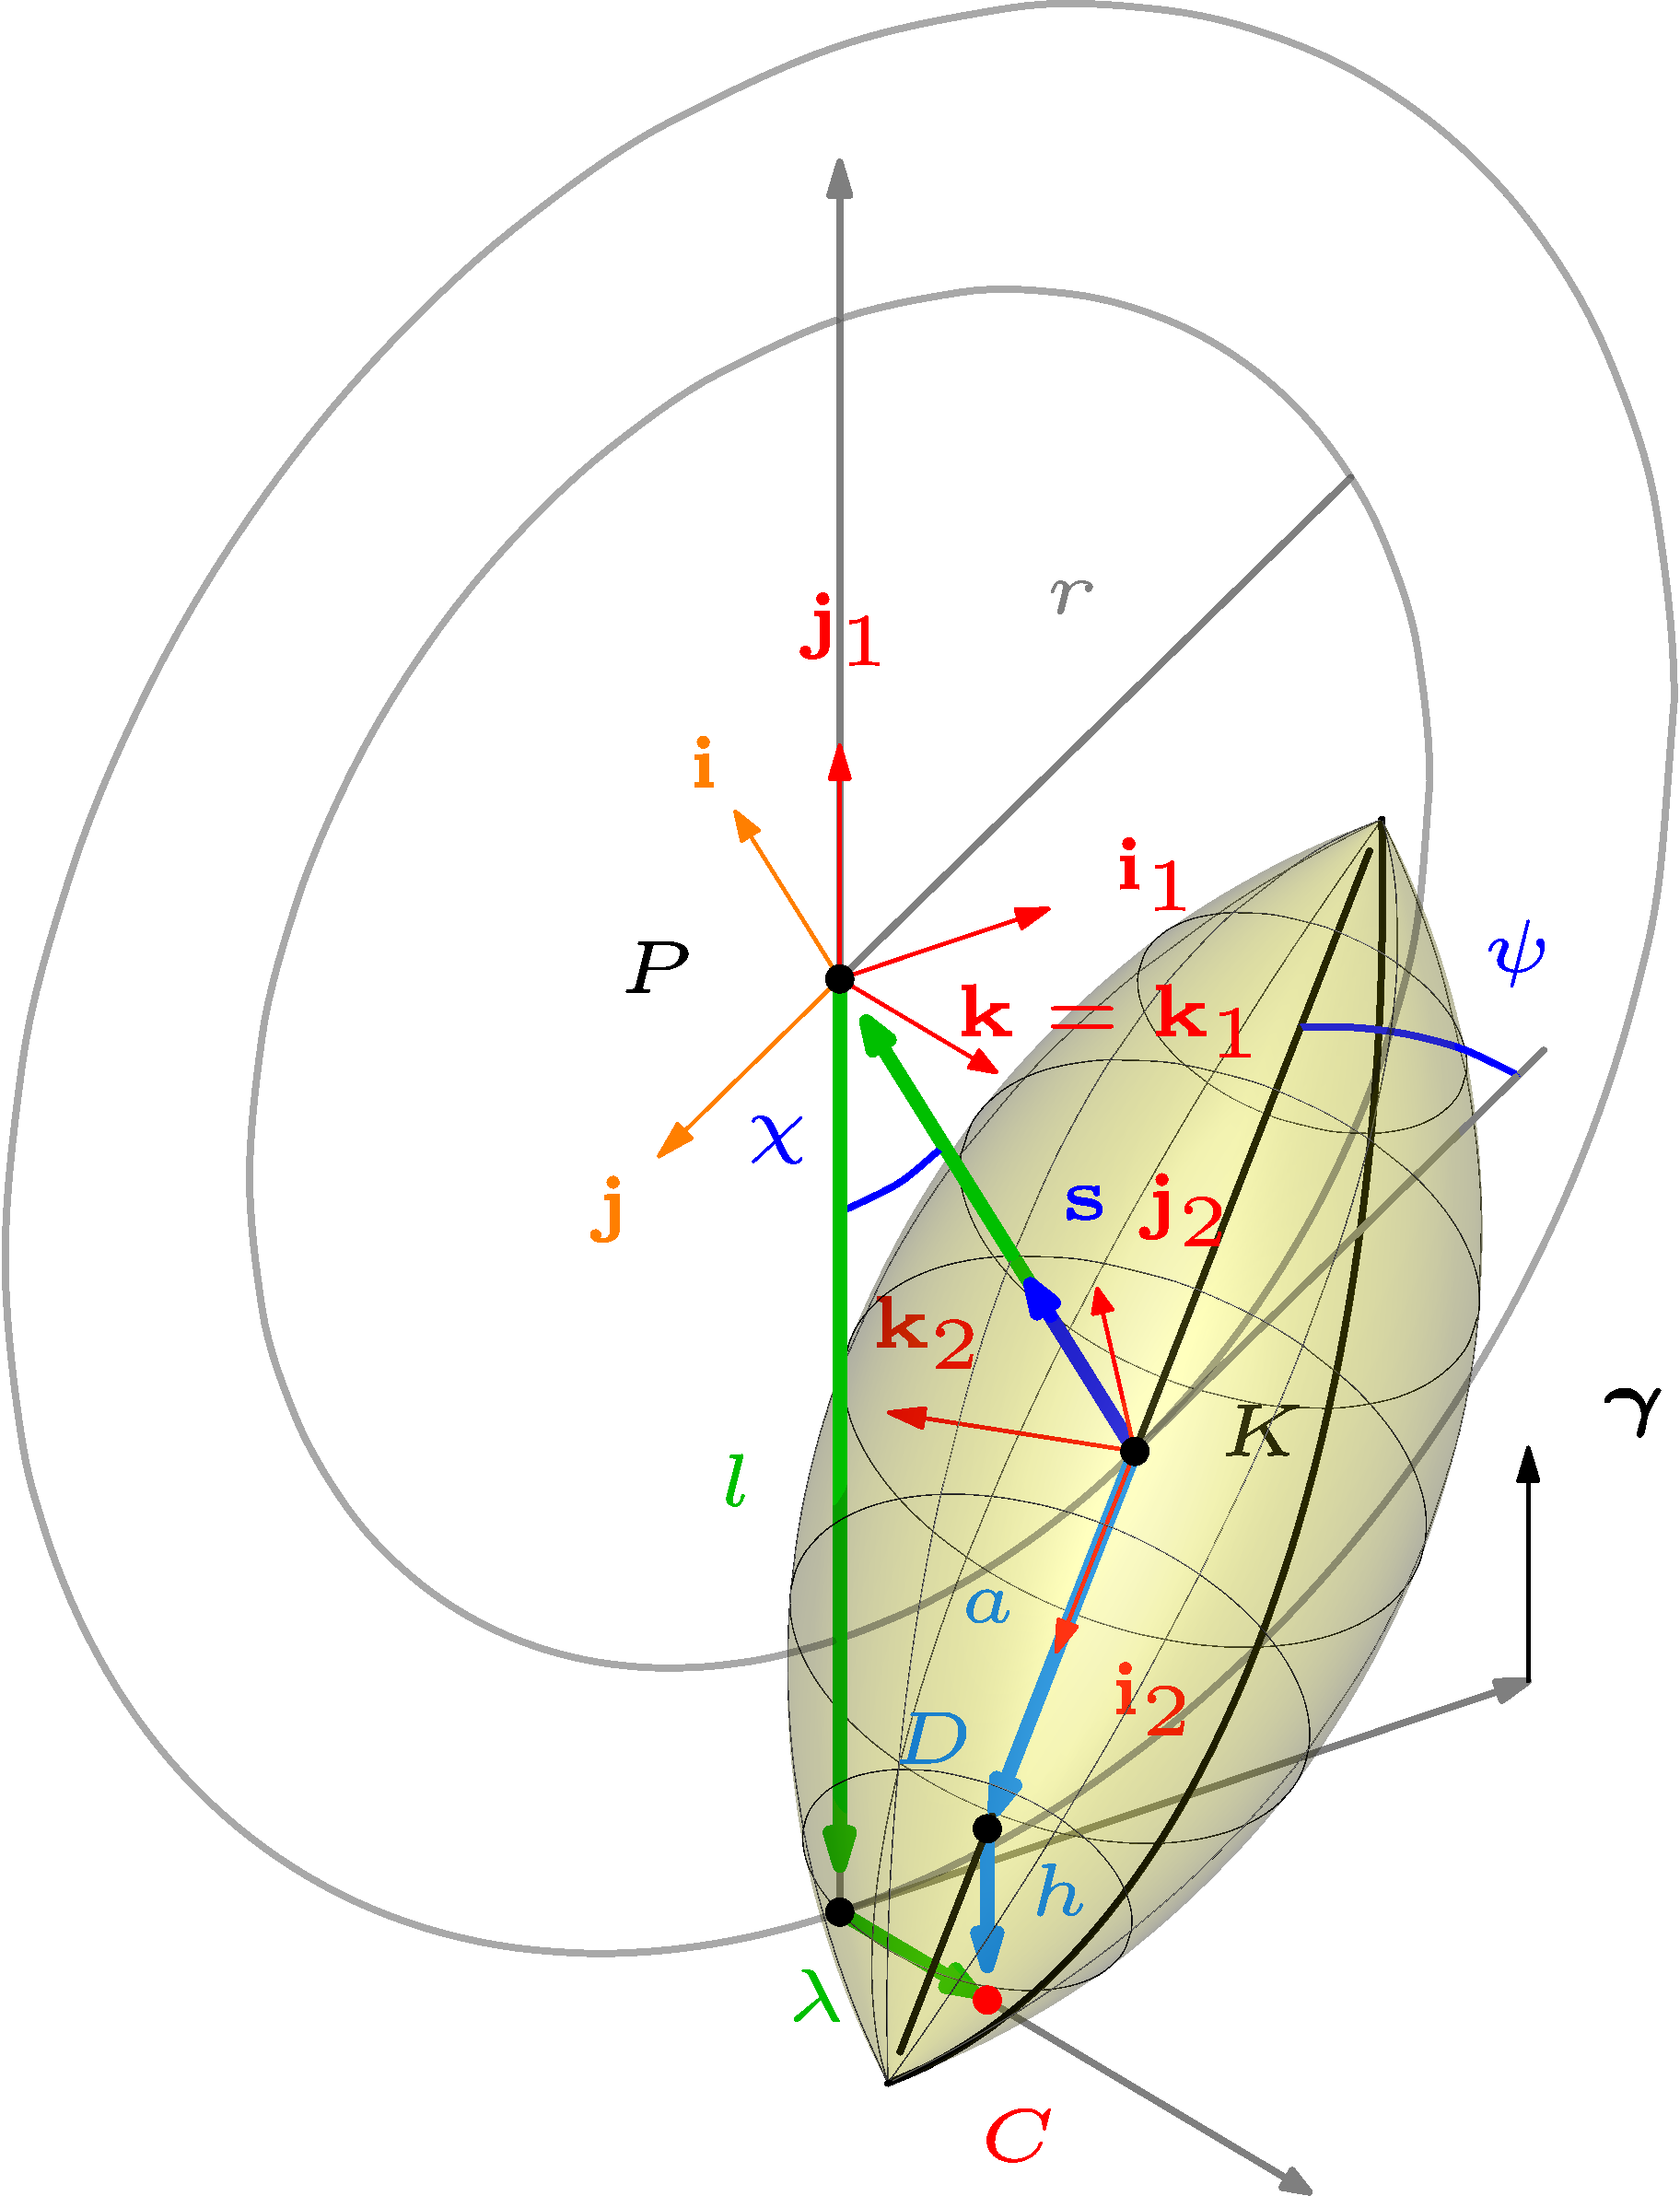
\includegraphics[width=\textwidth]{content/pic/asypng/pic_mecanum.png}
                    % \asyinclude[width=\textwidth]{content/pic/asy/pic_mecanum.asy}
                    \label{ContactScheme}
                \end{figure}
            \endminipage
            \quad
            \minipage{0.5\textwidth}
                $$ \vec{r}_C = \vec{r}_K + r\vec{s} - l\vec{e}_z + \lambda\vec{k}_1 $$
                $$ \lambda = \ddfrac{\left(r\vec{s} - l\vec{e}_z\right)\cdot\vec{k}_2}{ \vec{k}_1\cdot\vec{k}_2} $$
                $$ \vec{v}_C = \vec{v}_K + [ \vec{\omega}_{\text{рол}}, \overrightarrow{KC} ] $$
                Ролик находится в контакте $\iff$ $\vec{s} \cdot \vec{e}_z < \cos\ddfrac{\pi}{n} $ и $ z_C < l $. Тогда используются уравнения:
                $$ \vec{v}_C \cdot \vec{e}_z = 0 $$
                $$ \vec{R}_{\text{к}} = \vec{F}_{\text{тр}} + N\vec{e}_z $$
                Иначе $ \vec{R}_{\text{к}} = \vec{0} $
            \endminipage
            \vspace{10pt}
        }
    }
    
\end{myposter}
